\PassOptionsToPackage{unicode=true}{hyperref} % options for packages loaded elsewhere
\PassOptionsToPackage{hyphens}{url}
%
\documentclass[11pt,ignorenonframetext,]{beamer}
\usepackage{pgfpages}
\setbeamertemplate{caption}[numbered]
\setbeamertemplate{caption label separator}{: }
\setbeamercolor{caption name}{fg=normal text.fg}
\beamertemplatenavigationsymbolsempty
% Prevent slide breaks in the middle of a paragraph:
\widowpenalties 1 10000
\raggedbottom
\setbeamertemplate{part page}{
\centering
\begin{beamercolorbox}[sep=16pt,center]{part title}
  \usebeamerfont{part title}\insertpart\par
\end{beamercolorbox}
}
\setbeamertemplate{section page}{
\centering
\begin{beamercolorbox}[sep=12pt,center]{part title}
  \usebeamerfont{section title}\insertsection\par
\end{beamercolorbox}
}
\setbeamertemplate{subsection page}{
\centering
\begin{beamercolorbox}[sep=8pt,center]{part title}
  \usebeamerfont{subsection title}\insertsubsection\par
\end{beamercolorbox}
}
\AtBeginPart{
  \frame{\partpage}
}
\AtBeginSection{
  \ifbibliography
  \else
    \frame{\sectionpage}
  \fi
}
\AtBeginSubsection{
  \frame{\subsectionpage}
}
\usepackage{lmodern}
\usepackage{amssymb,amsmath}
\usepackage{ifxetex,ifluatex}
\usepackage{fixltx2e} % provides \textsubscript
\ifnum 0\ifxetex 1\fi\ifluatex 1\fi=0 % if pdftex
  \usepackage[T1]{fontenc}
  \usepackage[utf8]{inputenc}
  \usepackage{textcomp} % provides euro and other symbols
\else % if luatex or xelatex
  \usepackage{unicode-math}
  \defaultfontfeatures{Ligatures=TeX,Scale=MatchLowercase}
\fi
\usecolortheme{seahorse}
% use upquote if available, for straight quotes in verbatim environments
\IfFileExists{upquote.sty}{\usepackage{upquote}}{}
% use microtype if available
\IfFileExists{microtype.sty}{%
\usepackage[]{microtype}
\UseMicrotypeSet[protrusion]{basicmath} % disable protrusion for tt fonts
}{}
\IfFileExists{parskip.sty}{%
\usepackage{parskip}
}{% else
\setlength{\parindent}{0pt}
\setlength{\parskip}{6pt plus 2pt minus 1pt}
}
\usepackage{hyperref}
\hypersetup{
            pdftitle={Race, Class, and Transit Oriented Development},
            pdfauthor={Thelonious Goerz},
            pdfborder={0 0 0},
            breaklinks=true}
\urlstyle{same}  % don't use monospace font for urls
\newif\ifbibliography
\usepackage{graphicx,grffile}
\makeatletter
\def\maxwidth{\ifdim\Gin@nat@width>\linewidth\linewidth\else\Gin@nat@width\fi}
\def\maxheight{\ifdim\Gin@nat@height>\textheight\textheight\else\Gin@nat@height\fi}
\makeatother
% Scale images if necessary, so that they will not overflow the page
% margins by default, and it is still possible to overwrite the defaults
% using explicit options in \includegraphics[width, height, ...]{}
\setkeys{Gin}{width=\maxwidth,height=\maxheight,keepaspectratio}
\setlength{\emergencystretch}{3em}  % prevent overfull lines
\providecommand{\tightlist}{%
  \setlength{\itemsep}{0pt}\setlength{\parskip}{0pt}}
\setcounter{secnumdepth}{0}

% set default figure placement to htbp
\makeatletter
\def\fps@figure{htbp}
\makeatother


\title{Race, Class, and Transit Oriented Development}
\providecommand{\subtitle}[1]{}
\subtitle{\emph{Examining high-income demographic change after light rail transit}}
\author{Thelonious Goerz}
\providecommand{\institute}[1]{}
\institute{Dept. of Sociology\\
Johns Hopkins University}
\date{}

\begin{document}
\frame{\titlepage}

\begin{frame}{Outline}
\protect\hypertarget{outline}{}

\begin{itemize}
\tightlist
\item
  Background and prior research
\item
  Seattle case study
\item
  Methods and data
\item
  Descriptive and statistical results
\item
  Conclusion
\end{itemize}

\end{frame}

\begin{frame}{Motivation}
\protect\hypertarget{motivation}{}

\begin{itemize}
\tightlist
\item
  How and where people move have been a core questions in urban
  sociology and poverty research for years.

  \begin{itemize}
  \tightlist
  \item
    These moves have consequences for various aspects of life:
    wellbeing, economic status.
  \end{itemize}
\end{itemize}

\textbf{Therefore, it makes sense to study the most vulnerable
populations, right?}

\end{frame}

\begin{frame}{Motivation}
\protect\hypertarget{motivation-1}{}

\textbf{Well, sort of.}

\begin{itemize}
\tightlist
\item
  I argue an asymmetric focus on studying the movement patterns of
  low-income residents in changing neighborhoods has left open
  theoretical and empirical gaps for researchers.
\end{itemize}

\end{frame}

\begin{frame}{Background: Theory}
\protect\hypertarget{background-theory}{}

\begin{itemize}
\tightlist
\item
  Social scientists are interested in the effects of gentrification on
  urban demographic patterns.

  \begin{itemize}
  \tightlist
  \item
    In recent years, it has been linked to major urban re-investment
    projects, such as Light Rail Transit.
  \item
    So, transit is a good proxy for gentrification, neighborhood change,
    and associated ideas.
  \end{itemize}
\end{itemize}

\textbf{Why does studying transit matter?}

\end{frame}

\begin{frame}{Background: Theory}
\protect\hypertarget{background-theory-1}{}

\textbf{Seattle and many other cities are increasingly turning to Light
Rail Transit (LRT) as a way to manage growth, promote green travel
initiatives, and reduce congestion.}

\begin{itemize}
\tightlist
\item
  Manage the tech boom in WA.
\item
  Significant in-migration.
\item
  Population growth.
\end{itemize}

\end{frame}

\begin{frame}{The Present Study}
\protect\hypertarget{the-present-study}{}

\textbf{In Seattle:}

\begin{itemize}
\tightlist
\item
  The Link Light Rail has been in development since 1996 when it was
  approved.

  \begin{itemize}
  \tightlist
  \item
    Construction began in 2003 and a majority of stations opened in
    2009.
  \item
    As of 2021 there are 14 stations.
  \item
    There are currently north and south expansions in development to
    2036.
  \end{itemize}
\end{itemize}

\textbf{As a consequence:}

\begin{itemize}
\tightlist
\item
  There are puzzling trends going on.

  \begin{itemize}
  \tightlist
  \item
    Hess (2020) finds dramatic increases in non-Hispanic White residents
    after LRT in Seattle.
  \item
    Declines in Asian and Hispanic residents after LRT.
  \end{itemize}
\end{itemize}

\textbf{How is this happening?}

\end{frame}

\begin{frame}{Background: Income and mobility}
\protect\hypertarget{background-income-and-mobility}{}

\textbf{Conventional wisdom suggests that neighborhoods change through
low-income displacement.}

\begin{itemize}
\item
  But, low-income residents are often much less mobile than
  middle-income and higher-income residents (Freeman 2005).
\item
  However, there is evidence to suggest that middle and upper income
  residents are far more mobile:

  \begin{itemize}
  \tightlist
  \item
    Ding et al. (2016): Increases in high credit score individuals'
    mobility in gentrified neighborhoods.
  \item
    Bartholemew and Ewing (2017): Disamenity effect in neighborhoods
    with urban development, homeowners moving out.
  \item
    Martin and Beck (2011): Higher status non-homeowners may be moving
    out of gentrified neighborhoods.
  \end{itemize}
\end{itemize}

\end{frame}

\begin{frame}{The Present Study}
\protect\hypertarget{the-present-study-1}{}

\begin{itemize}
\tightlist
\item
  The demographic trends in Seattle are not consistent with patterns of
  socioeconomic mobility in changing neighborhoods.

  \begin{itemize}
  \tightlist
  \item
    Often low-income groups are declining.
  \item
    But, statistically these groups are not as mobile.
  \end{itemize}
\end{itemize}

\textbf{Where is this demographic change happening on average?}

\end{frame}

\begin{frame}{Hypothesis}
\protect\hypertarget{hypothesis}{}

\begin{itemize}
\tightlist
\item
  \textbf{This study argues that middle and high income groups are the
  primary forces shifting neighborhood racial composition in LRT
  neighborhoods because of their capacity to move.}
\end{itemize}

\end{frame}

\begin{frame}{Methods}
\protect\hypertarget{methods}{}

\begin{itemize}
\tightlist
\item
  Time series data for 135 census tracts (Seattle, N = 540) and 24 LRT
  treated tracts {[}1990-2015{]}:

  \begin{itemize}
  \tightlist
  \item
    Income (by race), demographic variables, and controls.
  \item
    American Community Survey, Decennial Census Long Form, Hess (2020).
  \end{itemize}
\item
  Difference in difference (comparative counterfactual design)

  \begin{itemize}
  \tightlist
  \item
    Quasi-experiment where:

    \begin{itemize}
    \tightlist
    \item
      We can estimate causality.
    \item
      Gain insights about what would have happened if (+ LRT) or (-LRT).
    \end{itemize}
  \end{itemize}
\end{itemize}

\end{frame}

\begin{frame}{Descriptive Analysis}
\protect\hypertarget{descriptive-analysis}{}

\begin{figure}

{\centering 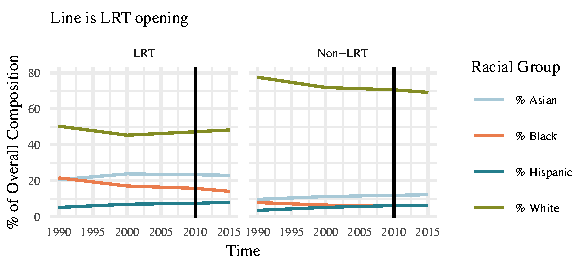
\includegraphics{csde_talk_files/figure-beamer/unnamed-chunk-3-1} 

}

\caption{Comparison of Percent of Each Racial Group Over Time in Seattle}\label{fig:unnamed-chunk-3}
\end{figure}

\end{frame}

\begin{frame}{Descriptive Analysis}
\protect\hypertarget{descriptive-analysis-1}{}

\begin{figure}

{\centering 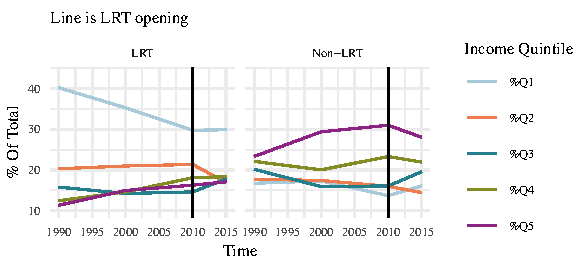
\includegraphics{csde_talk_files/figure-beamer/unnamed-chunk-4-1} 

}

\caption{Comparison of Income Quintiles in Seattle Census Tracts Over Time}\label{fig:unnamed-chunk-4}
\end{figure}

\end{frame}

\begin{frame}{Statistical Analysis: DID of racial composition}
\protect\hypertarget{statistical-analysis-did-of-racial-composition}{}

\begin{figure}
\centering
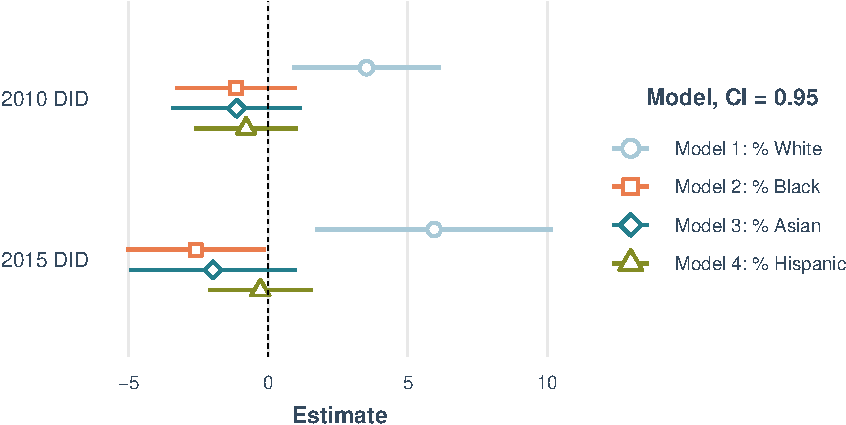
\includegraphics{csde_talk_files/figure-beamer/unnamed-chunk-9-1.pdf}
\caption{DID estimates of LRT effect on racial group percent}
\end{figure}

\end{frame}

\begin{frame}{Statistical Analysis: DID for income composition}
\protect\hypertarget{statistical-analysis-did-for-income-composition}{}

\begin{figure}
\centering
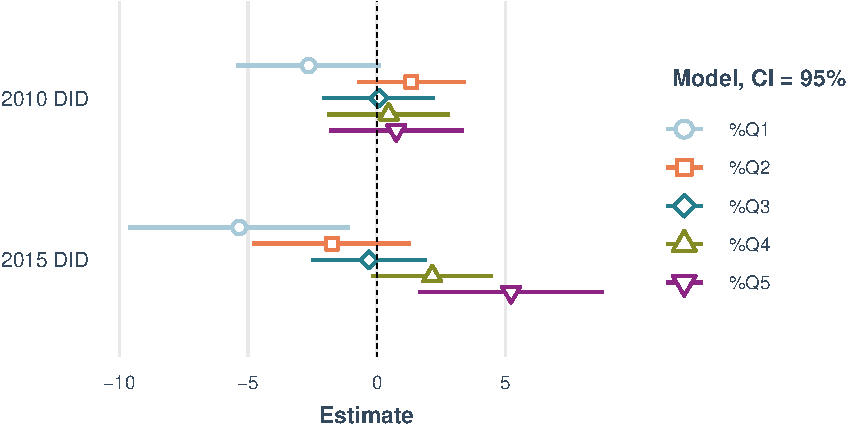
\includegraphics{csde_talk_files/figure-beamer/unnamed-chunk-11-1.pdf}
\caption{DID estimates of LRT effect on income quintile percent}
\end{figure}

\end{frame}

\begin{frame}{Conclusions}
\protect\hypertarget{conclusions}{}

\begin{itemize}
\tightlist
\item
  5 years after LRT, neighborhoods experience dramatic increases in
  white residents, and declining or stagnant non-white groups.
\item
  5 years after LRT, there is shift in the income distribution tending
  toward the highest quintile earners.\\
\item
  This suggests that income is an important factor in how demographics
  in Seattle are changing.
\item
  Income patterns are consistent with my hypothesis that dramatic shifts
  in income could be moving the composition.
\item
  But it is not clear how this change may vary by racial group.
\end{itemize}

\end{frame}

\begin{frame}{Limitations}
\protect\hypertarget{limitations}{}

\begin{itemize}
\tightlist
\item
  The ACS and census report compositional estimates so understanding how
  distribution changes translate to in and out migration flows is
  tricky.
\item
  Prediction of Black racial and economic trends can be subject to a lot
  of uncertainty.\footnote<.->{Data and full analysis provided on
    request. Email:
    \href{mailto:tgoerz99@uw.edu}{\nolinkurl{tgoerz99@uw.edu}}}

  \begin{itemize}
  \tightlist
  \item
    Small counts in ACS sample.
  \item
    Low levels of Black population overall in Seattle.
  \end{itemize}
\item
  DID modeling assumptions may not be met in this case.\footnote<.->{Parallel
    trends and endogeneity are issues, but beyond the scope of the
    presentation.}
\end{itemize}

\end{frame}

\begin{frame}{References}
\protect\hypertarget{references}{}

\fontsize{7pt}{7.2}\selectfont

Bartholomew, Keith, and Reid Ewing. 2011. ``Hedonic Price Effects of
Pedestrian- and Transit-Oriented Development.'' Journal of Planning
Literature 26(1):18--34. doi: 10.1177/0885412210386540.

Bertrand, Marianne, Esther Duflo, and Sendhil Mullainathan. 2003. ``HOW
MUCH SHOULD WE TRUST DIFFERENCES-IN-DIFFERENCES ESTIMATES?'' 32.

Chapple, Karen, and Anastasia Loukaitou-Sideris. 2019. Transit-Oriented
Displacement or Community Dividends?

Ding, Lei, Jackelyn Hwang, and Eileen Divringi. 2016. ``Gentrification
and Residential Mobility in Philadelphia.'' Regional Science and Urban
Economics 61:38--51. doi: 10.1016/j.regsciurbeco.2016.09.004.

Understanding the Effects of Smarter Growth on Communities. Cambridge,
MA: The MIT Press. City of Seattle. 2019. Seattle 2035 Urban Growth
Strategy. City of Seattle.

Freeman, Lance. 2005. ``Displacement or Succession?: Residential
Mobility in Gentrifying Neighborhoods.'' Urban Affairs Review
40(4):463--91. doi: 10.1177/1078087404273341.

Hess, Chris L. 2020. ``Light-Rail Investment in Seattle: Gentrification
Pressures and Trends in Neighborhood Ethnoracial Composition.'' Urban
Affairs Review 56(1):154--87. doi: 10.1177/1078087418758959.

Martin, Isaac William, and Kevin Beck. 2018. ``Gentrification, Property
Tax Limitation, and Displacement.'' Urban Affairs Review 54(1):33--73.
doi: 10.1177/1078087416666959.

\end{frame}

\end{document}
